\part{Log4Server}

\section{A centralized reporting web application}
\label{sec:log4server}
The \logftailer{} project includes a web backend application that receives
notifications from the log4tailer clients, notifying in a web front page about
the status of the logs in several machines. The log4server is implemented using
the Django web framework and can run in any wsgi compliant web server, such as
Apache, Cherokee, Nginx or CherryPy, just to name a few. Basically, the clients
will register first to the server and then notify if any fatal, error, critical
or target logtrace has been found. 

A network diagram is showed in \autoref{fig:serverdiagram}.

\begin{figure}[hb]
\centering
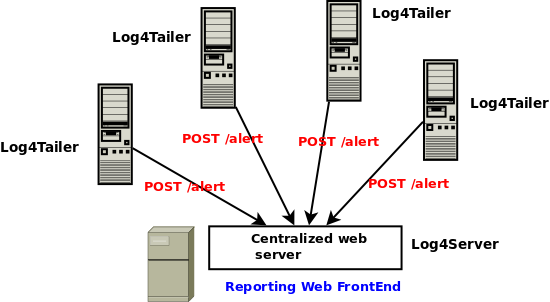
\includegraphics[scale=0.50]{serverdiagram.png}
\caption{Log4Server network diagram}\label{fig:serverdiagram}
\end{figure}


In the next section, we will describe the API that the log4server application implements and the 
one being used by the log4tailer poster notification.

\section{Log4Tailer compliant server}
\logftailer{} client has the poster notification that allows the tailer to communicate 
with a centralized web application, notifying it of possible problems from remote logs. 
The poster notification will first register the tailer client to the server, and next 
calls will be for alert notifications only.

\subsection{Log4Tailer server API REST interface}

The compliant API interface is as follows:

\subsubsection{Registration}

Log4tailer client registers to the server on startup when poster notification is provided.

\begin{flushleft}
 \begin{tabular}{|c|c|l|}
 \hline 
 \rowcolor{cyan} {\color{white} \textit{\textbf{HTTP Method}}} &  {\color{white} 
  \textit{\textbf{URL}}}  & {\color{white} 
 \textit{\textbf{Description}}}\\
 POST & /register/ & Log4tailer client registration to the server\\
 \hline
\end{tabular}
\end{flushleft}
The POST method will have in the body a JSON object with the following information:

\begin{itemize}
 \item logpath Full path of the log 
 \item hostname log's server hostname
\end{itemize}

\noindent
Upon a successul POST the server will reply a 201 CREATED answer.

\noindent
Example:

\begin{codeexample}

POST /register/

 \{``logpath'' : ``/var/log/messages'', ``logserver'' : ``localhost''\} 

RESPONSE

 \{``id'' : 3\} 

HTTP/1.1 201 CREATED.
\end{codeexample}

The id returned is the log identifier id.

\subsubsection{Unregistration}

Log4tailer client unregisters from the server ones it is stopped.

\begin{flushleft}
 \begin{tabular}{|c|c|l|}
 \hline 
 \rowcolor{cyan} {\color{white} \textit{\textbf{HTTP Method}}} &  {\color{white} 
  \textit{\textbf{URL}}}  & {\color{white} 
 \textit{\textbf{Description}}}\\
 POST & /unregister/ & Log4tailer client unregistration to the server\\
 \hline
\end{tabular}
\end{flushleft}
The POST method will have in the body a JSON object with the following information:

\begin{itemize}
 \item id log registration id 
\end{itemize}

\noindent
Upon a successul POST the server will reply a 200 OK answer

\noindent
Example:

\begin{codeexample}

POST /unregister/

 \{``id'' : 4 \}

RESPONSE

HTTP/1.1 200 OK.
\end{codeexample}

\subsubsection{Alerting}

\begin{flushleft}
 \begin{tabular}{|c|c|l|}
 \hline 
 \rowcolor{cyan} {\color{white} \textit{\textbf{HTTP Method}}} &  {\color{white} 
  \textit{\textbf{URL}}}  & {\color{white} 
 \textit{\textbf{Description}}}\\
 POST & /alerts/ & New alert has been found.\\
 \hline
\end{tabular}
\end{flushleft}
The POST method will have in the body a JSON object with the following information:

\begin{itemize}
 \item logtrace logtrace that triggered the alert.
 \item level level of the aforementioned logtrace.
 \item log log where the logtrace belongs to.
    \begin{itemize}
      \item logpath Full path of the log 
      \item hostname log's server hostname
    \end{itemize}
\end{itemize}
Upon a successul POST the server will reply a 201 CREATED answer.

\noindent
Example:

\begin{codeexample}

POST /alerts/

 \{``logtrace'' : ``This is an error trace'', 
   ``loglevel'' : ``error'',
   ``log'' : \{``id'' : ``logid'', ``logpath'' : ``/var/log/messages'', ``logserver'': 
``192.168.1.1''\}\} 

RESPONSE

HTTP/1.1 201 CREATED.
\end{codeexample}

\subsubsection{Status}

\begin{flushleft}
 \begin{tabular}{|c|c|l|}
 \hline 
 \rowcolor{cyan} {\color{white} \textit{\textbf{HTTP Method}}} &  {\color{white} 
  \textit{\textbf{URL}}}  & {\color{white} 
 \textit{\textbf{Description}}}\\
 GET & /alerts/status & Status of the log files.\\
 \hline
\end{tabular}
\end{flushleft}
It returns all log traces triggered along with the log and server they belong to. The 
date when it happened is reported as well. The results are paginated in reverse
order, the newest first.

\noindent
Example:

\begin{codeexample}

GET /alerts/status

RESPONSE

HTTP/1.1 200 OK.
\end{codeexample}


\noindent
If you go to /alerts/status in your web browser, you would see something as showed in  
\autoref{fig:logstatus}.

\begin{figure}[ht]
%\centering
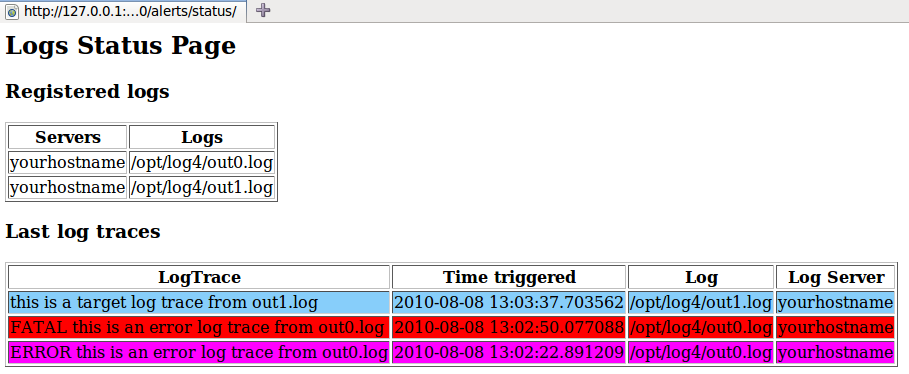
\includegraphics[scale=0.50]{logstatus.png}
\caption{Log4Server status web reporting}\label{fig:logstatus}
\end{figure}

\section{Log4Server deployment}
Log4Server is implemented using the Django web framework. It persists alertable
log traces into a database for easy reporting and log4tailer client
registrations. 

The application uses buildout to manage all application dependencies and
deployment. By issuing the bin/buildout command, it will build a
log4server.wsgi file, that is the one that you will need to use when setting up
the web server. In this document, we will show the instructions on how to set
it up by using the Apache web server. 

\subsection{Building the wsgi file}

First of all, download the log4server distribution sources from googlecode
site. Untar the package and execute\footnote{The project provides a Makefile
that executes the bin/buildout command for convenience. It can take a while, so 
relax and take a cup of tea.}:

\begin{cmd}
    make
\end{cmd}
If everything is fine\footnote{You need external internet connectivity, as it
will download all dependencies such as Django web framework in the current
directory.} you will see a directory called \emph{bin}. If you go
into that directory you will see a file called log4tailer.wsgi. 

\subsection{Apache configuration}
In a Debian system such as Ubuntu, you'll need to install Apache and
libapache2-mod-wsgi. Once installed, proceed as follows:

\begin{cmd}
    cd /etc/apache2/sites-available
\end{cmd}
and place a file called log4tailer.conf with the following contents:

\begin{config}
\begin{verbatim}

Listen 127.0.0.1:8000
<VirtualHost *:8000>
    WSGIDaemonProcess log4server processes=1 threads=5 display-name=%{GROUP}
    WSGIProcessGroup log4server
    WSGIScriptAlias / /path\_to\_thewsgi/log4server/bin/log4server.wsgi
</VirtualHost>

\end{verbatim}
\end{config}

Then, go to:

\begin{cmd}
    cd /etc/apache2/sites-enabled
\end{cmd}
and place a soft link to the previous created log4tailer.conf file:

\begin{cmd}
    ln -s ../sites-available/log4tailer.conf
\end{cmd}


\subsection{Deciding on database}

Log4Server needs a database in order to persist the alertable logtraces. 
Sqlite3, Mysql or PostGres should be, by far, enough. Actually, with just an
Sqlite3 would be just fine. Before starting starting the server, you should
sync the database the first time or any time that the database does not exist
already. In order to do that, execute the following command:

\begin{cmd}
   bin/log4server syncdb 
\end{cmd}
\emph{log4server} is just a wrapper for the \emph{manage.py} Django python
script. Make sure you setup \todo[size=\footnotesize,color=yellow]{should we
provide an etc settings.py? in buildout}.

\newpage
